\section{Problem Formulation}
%----------------------------------------------------------------------------------------%
In this section, we formulate the optimization problem which aims at online optimizing job dispatching decisions of all APs.
This kind of optimization problem falls into multi-agent planning problem, which considers a fully cooperative multi-agent system (MAS) and each agent shares the same utility function \needref{Craig Boutilie, 1999}.
In our problem, we focus on the real situation about communication overhead in MAS, where the system information is always stale due to periodic broadcast and \brdelay.
\needref{R.Nair, 2003} uses DEC-POMDP (Decentralized Partial-Observed MDP) framework to characterize the coordination among decentralized and partially observed multi-agent problem. The solution to its problem is of high complexity and requires extra information of \emph{belief states}.
Instead, we formulate the problem under standard MDP framework, which is with fully-observable information.
At the end of this section, we show that we could come up with decentralized algorithm under the global problem formulation heuristically. A low-complexity solution is also provided in the following section to alleviate the curse of dimensionality.
\delete{v4}{Reference list
    [1] "Sequential Optimality and Coordination in Multi-agent Systems", Craig Boutilie, 1999
    [2] "Taming Decentralized POMDPs: Towards Efficient Policy Computation for Multi-agent Settings", R.Nair, 2003
}

\subsection{System State and Dispatching Policy}
We formulate the multi-agent MDP problem from a global perspective, where each AP adopts the dispatching policy mapping from the global broadcast information $\Obsv^{\dagger}$.
% As each AP would always update its dispatching policy based on the latest broadcast information, the \brdelay{s} in each interval is also taken as a part of state information.
The relationship between \brdelay~and the policy update time points for different APs is depicted in Fig. \ref{fig:brd-trans}.

\accept{
    \begin{definition}[System State]
        The system state for the $t$-th broadcast interval is denoted as follows.
        \begin{align}
            \Stat({t}) \define \Paren{
                \Obsv^{\dagger}({t-1}), \Obsv^{\dagger}({t}), \mathcal{D}({t})
            },
        \end{align}
        where $\mathcal{D}({t}) \define \set{D_{1}({t}), \dots, D_{K}({t})}$ denotes the \brdelay~for each AP, $\Obsv^{\dagger}({t})$ denotes updated global information with the whole broadcast information, and $\Obsv^{\dagger}({t-1})$ denotes the stale global information.
    \end{definition}
}

\begin{figure}[ht]
    \centering
    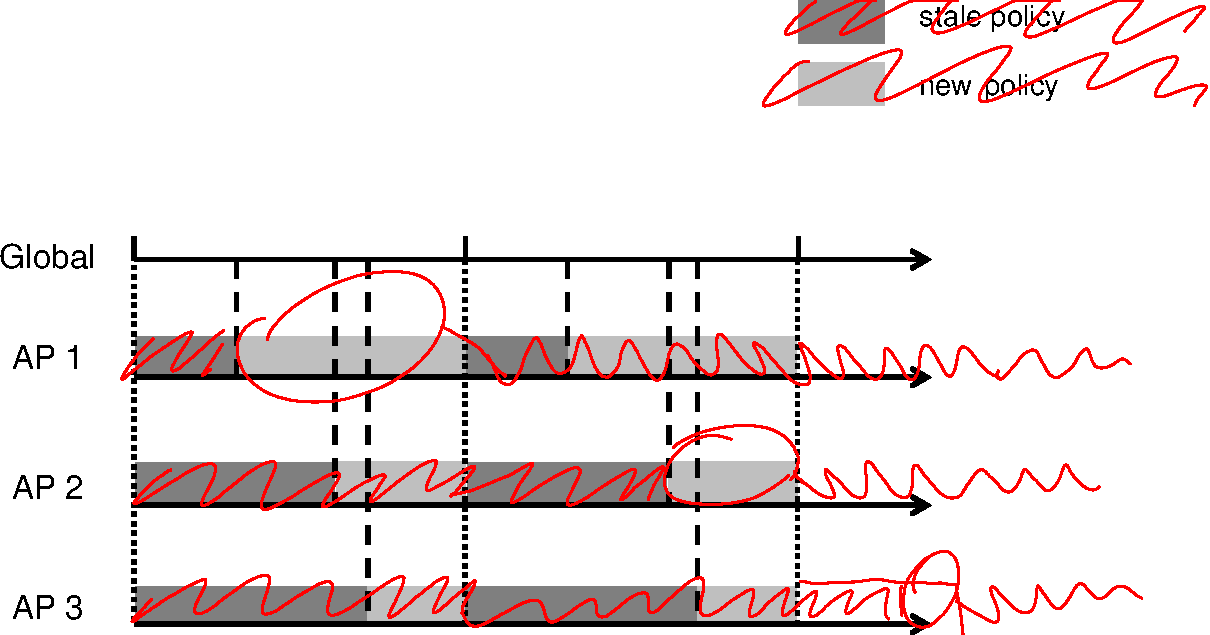
\includegraphics[width=0.80\textwidth]{brd-trans.pdf}
    \caption{Global System Transition with Partial Information-based Dispatching Decision}
    \label{fig:brd-trans}
\end{figure}

Based on the two phases of broadcast information in the system state, the system evolves with the joint actions of all APs.
Due to the different distributions of \brdelay~for each AP in one interval, APs use the stale policy in firstly and then update their policy based on latest information in random order.
The joint policy of all APs is defined as follows.
\accept{
    \begin{definition}[Joint Dispatching Policy]
        The joint dispatching policy $\Policy(\Stat({t}))$ over global system state $\Stat({t})$ which is defined as follows.
        \begin{align}
            \Policy^{\dagger}(\Stat(t)) \define \Brace{
                \Omega^{\dagger}_{1}(\Stat(t)), \dots, \Omega^{\dagger}_{K}(\Stat(t))
            },
        \end{align}
        where $\Omega^{\dagger}_{k}(\Stat({t}))$ denotes the independent policy for the $k$-th AP ($\forall k\in\apSet$) mapping from the global state. whose definition is given as follows.
        \begin{align}
            \Omega^{\dagger}_{k}\Paren{\Stat({t})} \define
            \begin{cases}
                {\Omega}_{k}( \Obsv_{k}({t-1}) ), &n <    D_{k}({t})
                \\
                {\Omega}_{k}( \Obsv_{k}({t}) ),   &n \geq D_{k}({t})
            \end{cases},
        \end{align}
        where $n$ denotes the index of time slot in the $t$-th interval. And we note that the individual policy ${\Omega}_{k}( \Obsv_{k}({t}) )$ would be adopted when the $k$-th AP receives the partial information ($t+D_{k}(t)$), and lasts until the time when the next partial broadcast information arrives ($t+1+D_{k}(t+1)$). The lasting time of one individual policy is un-deterministic. 
    \end{definition}
}
%----------------------------------------------------------------------------------------%

\subsection{The Optimization Problem}
In our system, each AP individually performs job dispatching decision, and coordinates in a fully cooperative manner sharing the same utility function.
We propose the jobs dispatching optimization problem with the target to minimize \emph{average response time} of all offloaded jobs in MEC system.
The \emph{average response time} is composed of uploading time from APs to edge servers, and queueing-and-service time on corresponding edge server. According to \emph{Little's Law}, the average response time of all jobs is equally as average number of jobs in system.

Due to the periodic information broadcasting, we collect the cost for counting numbers each interval, which could be seen as a uniform sampling at times lot scale.
Besides the cost counted for job response time, we further add penalty on jobs rejection on edge servers when the job submission is over the queue capacity limit. The penalty will be counted at the end of each broadcast interval.
The definition of the cost function is given as follows.
\begin{align}
    g^{\dagger}\Paren{\Stat({t}), \Policy^{\dagger}(\Stat({t}))} \define
        &\sum_{k\in\apSet} \sum_{m\in\esSet} \sum_{j\in\jSpace} \vec{R}^{(k)}_{m,j}({t})~+
        \nonumber\\
        &\sum_{m\in\esSet} \sum_{j\in\jSpace} \Brace{L_{m,j}({t}) + \beta \cdot \mat{I}[L_{m,j}({t})=L_{max}]},
\end{align}
where $\beta$ is the weight factor for job rejection penalty ($\beta \in (0,1)$).

\begin{problem}[Centralized Job Dispatching Problem]
    \begin{align}
        \min_{\Policy^{\dagger}} \lim_{T \to \infty}
            \mathbb{E}_{\Policy^{\dagger}}
                \Bracket{\sum_{t=1}^{T} \gamma^{t-1} g^{\dagger}\Paren{\Stat({t}), \Policy^{\dagger}(\Stat({t}))}|\Stat(1)},
    \end{align}
    where the cost is collected with a discount factor $\gamma$.
\end{problem}
According to \cite{sutton1998introduction}, the above problem could be solved by the following \emph{Bellman's equation}:
\begin{align}
    V^{\dagger}\Paren{\Stat({t})} =~&g^{\dagger}\Paren{\Stat({t})} + \gamma \min_{\Policy(\Stat({t}))}
        \nonumber\\
        &\sum_{\Stat({t+1})} \Pr\Brace{ \Stat({t+1})|\Stat({t}), \Policy(\Stat({t})) } \cdot V^{\dagger}\Paren{\Stat({t+1})}.
    \label{sp_0}
\end{align}
\accept{
    However, if we only update the individual policy of the $k$-th AP ($\forall k\in\apSet$) at one time, the Bellman's equation would reduce into the form as follows, where only the partial information for the $k$-th AP matters.
    \begin{align}
        V_{k}\Paren{\Obsv_{k}({t})} =& g_{k}(\Obsv_{k}(t)) +
        \gamma\min_{\Omega_{k}(\Obsv_{k}(t))}
        \nonumber\\
        &\sum_{\Obsv_{k}(t+1)} \Pr
        \Brace{ 
            \Obsv_{k}(t+1) | \Obsv_{k}(t), \Policy_{k}(t-1), \Omega_{k}(\Obsv_{k}(t))
        } \cdot V_{k}\Paren{\Obsv_{k}({t+1})},
    \end{align}
    where,
    \begin{align}
        g_{k}(\Obsv_{k}(t)) \define& \sum_{j\in\jSpace} \Brace{
            \sum_{k\in\mathcal{X}_{k}} \sum_{m\in\esSet_{k}} \vec{R}^{(k)}_{m,j}(t) +
            \sum_{m\in\esSet_{k}} \set{ L_{m,j}(t) + \beta \cdot \mat{I}[L_{m,j}(t)=L_{max}] }
        }
        \\
        \Policy_{k}(t-1) \define & \Brace{ \Omega_{k'}(\Obsv_{k'}(t-1)) | \forall k'\in\mathcal{X}_{k} }
    \end{align}
}
To better analyze the structure of the optimization problem, we decouple the transition function.
The expression of transition function in Eqn. (\ref{sp_0}) is given as follows.
\begin{lemma}[Transition Function Decoupling]
    The transition function in Bellman's equation could be decoupled on states of APs and edge servers, which will facilitate the approximated value function expression in the following section.
    The decoupled transition function for Eqn. (\ref{sp_0}) is given as follows.
    \begin{align}
        & \Pr\Brace{ \Stat({t+1})|\Stat({t}), \Policy(\Stat({t})) }
        \nonumber\\
        =& \Pr\{\mathcal{D}({t+1})\} \times \Pr\Brace{ \Obsv({t+1})|\Obsv({t}), \Policy(\Stat({t}))}
        \nonumber\\
        =& \Pr\{\mathcal{D}({t+1})\} \times \prod_{k\in\apSet}\prod_{m\in\esSet}\prod_{j\in\jSpace}
                \Pr\Brace{
                    \vec{R}^{(k)}_{m,j}({t+1}) | \vec{R}^{(k)}_{m,j}({t}),
                    \Policy(\Stat({t}))
                }  
            \nonumber\\
            & \times \prod_{m\in\esSet}\prod_{j\in\jSpace}
                \Pr\Brace{
                    Q_{m,j}({t+1})|Q_{m,j}({t}), \mathcal{R}({t}), \Policy(\Stat({t}))
                }.
    \end{align}
\end{lemma}
\begin{proof}
    Proof deleted.
\end{proof}

The transition function, \fixit{except for standalone probability distribution $\Pr\{\mathcal{D}({t})\}$,} is consisted of two parts of state transitions on APs and edge servers, respectively.
To efficiently express the state transition, we further elaborate the distribution probability of the state vector as the corresponding probability vector, and perform the state transition with the transition matrix.
For state transition of APs inside one interval, we denote $\vecG{\Theta}^{(k)}_{m,j}(t,n)$ and ${\Gamma}^{(k)}_{m,j}(t,n)$ as probability vector and transition matrix, respectively, for $\vec{R}^{(k)}_{m,j}(t,n)$ of the $j$-th type of job uploading from the $k$-th AP to the $m$-th edge server ($\forall k\in\apSet, m\in\esSet, j\in\jSpace$). The definition is given as follows.
\begin{align}
    \Gamma^{(k)}_{m,j}(t,n) \define
    \begin{bmatrix}
        1 & \bar{p}^{(k)}_{m,j,0} &                       &        &                           \\
          & 0                     & \bar{p}^{(k)}_{m,j,1} &        &                           \\
          &                       & \ddots                & \ddots &                           \\
          &                       &                       & \ddots & \bar{p}^{(k)}_{m,j,\Xi-1} \\
          &                       &                       &        & 0                         \\
    \end{bmatrix},
    \vecG{\Theta}^{(k)}_{m,j}(t,n) \define
    \begin{bmatrix}
        \theta^{(k)}_{m,j,0}(t,n) \\
        \theta^{(k)}_{m,j,1}(t,n) \\
        \vdots \\
        \vdots \\
        \theta^{(k)}_{m,j,\Xi}(t,n)
    \end{bmatrix},
\end{align}
where $p^{(k)}_{m,j,\xi} \define \Pr\{U^{(k)}_{m,j} < (\xi+1) | U^{(k)}_{m,j}>\xi\}$ and $\bar{p}^{(k)}_{m,j,\xi} = 1 - p^{(k)}_{m,j,\xi}$ denote the probability of staying and offloading, respectively; $\theta^{(k)}_{m,j,\xi}(t,n) \define \Pr\{R^{(k)}_{m,j,\xi}(t,n) = 1\}$ denotes the distribution probability of existing job in the corresponding counters of the AP ($\forall \xi=0,\dots,\Xi$).

And we note that $\theta^{(k)}_{m,j,0}(t,n)$ is purely determined by the arrival process and dispatching policy of the $j$-th type of job on the $k$-th AP, i.e. $\theta^{(k)}_{m,j,0}(t,n) = \lambda_{k,j} I[\omega_{k,j}(t,n) = m]$, where $I[\cdot]$ is the indicator function.
Hence, the state transition between adjacent interval from $\vecG{\Theta}^{(k)}_{m,j}(t+1)$ to $\vecG{\Theta}^{(k)}_{m,j}(t)$ is composed of two-phase policy separated by $D_k(t)$, which could be expressed as follows.
\begin{align}
    \vecG{\Theta}^{(k)}_{m,j}(t, D_{k}(t)) &= (\Gamma^{(k)}_{m,j})^{D_{k}(t)} \times \vecG{\Theta}^{(k)}_{m,j}(t),
    \nonumber\\
    \vecG{\Theta}^{(k)}_{m,j}({t+1}) &= (\Gamma^{(k)}_{m,j})^{N-D_{k}(t)} \times \vecG{\Theta}^{(k)}_{m,j}(t, D_{k}(t)).
\end{align}

For state transition of edge servers, we denote $\vecG{\mu}_{m,j}$ and $P_{m,j}$ as probability vector and transition matrix, respectively, for $Q_{m,j}$ of the $j$-th job processing on the $m$-th edge server ($\forall m\in\esSet, j\in\jSpace$). The definition of the probability vector $\vecG{\mu}_{m,j}(t,n)$ at the $n$-th time slot in the $t$-the interval is given as follows.
\begin{align}
    \vecG{\mu}_{m,j}(t,n) \define 
    \begin{bmatrix}
        &\Pr\{L_{m,j}(t,n)=0,   &        & \eta_{m,j}(t,n)=0\} \\
        &\Pr\{L_{m,j}(t,n)=0,   &        & \eta_{m,j}(t,n)=1\} \\
        &                       & \vdots & \\
        &\Pr\{L_{m,j}(t,n)=0,   &        & \eta_{m,j}(t,n)=\mathcal{C}_{m,j}-1\} \\
        &\Pr\{L_{m,j}(t,n)=1,   &        & \eta_{m,j}(t,n)=0\} \\
        &                       & \vdots & \\
        &\Pr\{L_{m,j}(t,n)=L_{max}, &        & \eta_{m,j}(t,n)=\mathcal{C}_{m,j}-1\}
    \end{bmatrix}
\end{align}
However, the expression of transition matrix $P_{m,j}$ is more complex. Firstly, we notice that in the transition function of edge server, the distribution of offloading number of jobs from all APs in the interval contributes to the job arrival process on edge server as $\mathcal{R}(t)$. We denote the offloading matrix $\bar{\Gamma}^{(k)}_{m,j}$ from each AP to the $m$-th edge server as follows.
\begin{align}
    \bar{\Gamma}^{(k)}_{m,j}(t,n) \define
    \begin{bmatrix}
        0 & p^{(k)}_{m,j,0} &                 &        &                     \\
          & 0               & p^{(k)}_{m,j,1} &        &                     \\
          &                 & \ddots          & \ddots &                     \\
          &                 &                 & \ddots & p^{(k)}_{m,j,\Xi-1} \\
          &                 &                 &        & 1                   \\
    \end{bmatrix},
\end{align}
And the offloading number vectors are denoted as follows.
\begin{align}
    \vecG{\rho}^{(k,+)}_{m,j}({t,n}) &\define \bar{\Gamma}^{(k)}_{m,j} \times \vecG{\theta}^{(k)}_{m,j}({t,n}),
\end{align}
and the arrival number at the $n$-th time slot in the $t$-th interval on the $m$-th server is $\sum_{k\in\apSet} \vecG{\rho}^{(k,+)}_{m,j}({t,n})$,
The dimension of the compounded vector would be un-acceptable, as the increase of AP numbers would result into exponential expansion of dimensionality.
Thus we rewrite the arrival process on edge server with small probability approximation, i.e. there would be at most one job arring in one time slot, with the probability as the expected arrival rate of the original distribution. The explicit definition of the approximate arriving probability $\beta_{m,j}({t,n})$ is given as follows.
\begin{align}
    {\beta}_{m,j}({t,n}) &\define \sum_{k\in\mathcal{K}} \sum_{\xi=0,\dots,\Xi-1} \mathbb{E}[\vecG{\rho}^{(k,+)}_{m,j,\xi}({t,n})]
    \label{eqn_0}
\end{align}
We could prove that the error due to approximation is negligible.
\begin{lemma}[Small Probability Approximation]
    The probability distribution of $\sum_{k\in\apSet} \vecG{\rho}^{(k,+)}_{m,j}({t,n})$ could be approximated with Bernoulli arrival process with the same expected arrival rate denoted as ${\beta}_{m,j}({t,n})$.
\end{lemma}
\begin{proof}
    \fixit{
        We notice that the job arrival distribution ${\beta}_{m,j}({t})$ is given by $\mathcal{R}({t})$, and the departure rate in one slot is deterministic as $1/N$.
        Thus the expectation of ${\beta}$ would be always far more smaller than $1$ as composed of all $K$ AP nodes.
        We take approximation on ${\beta}$ as Bernoulli distribution in each time slot.
    }
\end{proof}

Thus we could obtain the time-variant transition matrix composed of multiple transition matrix $P_{m,j}(\beta({t,n}))$ in all the time slots in $i$-th interval as follows.
\begin{align}
    \vecG{\nu}({t,n+1}) &= P_{m,j}\Paren{\beta_{m,j}({t,n})} \vecG{\nu}({t,n})
    % \label{eqn_3}
    \\
    \vecG{\nu}({t+1}) &= \prod_{n=0,\dots,N-1} P_{m,j}\Paren{\beta_{m,j}({t,n})} \vecG{\nu}({t}),
    \label{eqn_4}
\end{align}

However, after the state decomposition, the action space would still be exponentially expanded with respect to the number of APs and edge servers.
We could not use traditional \emph{policy iteration} or \emph{value iteration} algorithm \cite{sutton1998introduction} for unacceptable computational complexity.
So in next section, to alleviate curse of dimensionality, we introduce baseline dispatching policy to approximate the value function, and then carry out one-step iteration \st{in a polling manner} to obtain a better value function approximation.
%----------------------------------------------------------------------------------------%

\delete{v4}{
    Outline:
    \begin{itemize}
        \item and $\Policy$ is optimized policy globally always with full-state information available.
        \item \needref{R.Nair, 2003} uses DEC-POMDP (Decentralized Partial-Observed MDP) framework to characterize the coordination among decentralized and partially observed multi-agent problem. The solution to its problem is of high complexity and requires extra information;
        \item thus we come up with sub-optimal solution to the Bellman equation; (where the lower and upper bound are analytically obtained;
        \item The \emph{exhaustive-JESP} algorithm implies, each AP only update the policy of itself, and consider other APs' policy fixed in the environment.
        \item Remark: Assume that we solve the sub-problems following the order of index of AP set, and then substitute the solution to the $k$-th problem to the $(k+1)$-th problem ($\forall k\in\apSet$).
              Apparently, we could achieve a sub-optimal solution of all APs which is upper bounded by the solution to the original problem.
        \item We restrict out observation in solution part, and just leverage the structure of the above centralized optimization problem.
        \end{remark}
    \end{itemize}
}